\documentclass[aspectratio=169, 11pt]{beamer}
% \documentclass[aspectratio=169, 11pt, handout]{beamer}

% ── Theme ──
\usetheme{Madrid}
\usecolortheme{default}
\setbeamertemplate{navigation symbols}{}
\setbeamertemplate{footline}{%
  \leavevmode\hbox{%
    \begin{beamercolorbox}[wd=.333333\paperwidth,ht=2.5ex,dp=1ex,center]{author in head/foot}%
      \usebeamerfont{author in head/foot}\insertshortauthor
    \end{beamercolorbox}%
    \begin{beamercolorbox}[wd=.333333\paperwidth,ht=2.5ex,dp=1ex,center]{title in head/foot}%
      \usebeamerfont{title in head/foot}\insertshorttitle
    \end{beamercolorbox}%
    \begin{beamercolorbox}[wd=.333333\paperwidth,ht=2.5ex,dp=1ex,right]{date in head/foot}%
      \usebeamerfont{date in head/foot}\insertframenumber{} / \inserttotalframenumber\hspace*{2ex}
    \end{beamercolorbox}}}

% ── Packages ──
\usepackage{amsmath,amssymb}
\usepackage{booktabs}
\usepackage{xcolor}
\usepackage{colortbl}
\usepackage{tikz}
\usetikzlibrary{arrows.meta, positioning}
\usetikzlibrary{calc} 

% ── Colors ──
\definecolor{sbgreen}{HTML}{00704A}
\definecolor{warnred}{HTML}{CC0000}
\definecolor{noteblue}{HTML}{2060A0}

% ── Commands ──
\newcommand{\E}{\mathbb{E}}
\newcommand{\Var}{\mathrm{Var}}
\newcommand{\Cov}{\mathrm{Cov}}
\newcommand{\SE}{\mathrm{SE}}
\newcommand{\Prob}{\mathrm{Pr}}
\newcommand{\indep}{\perp\!\!\!\perp}
\DeclareMathOperator{\plim}{plim}

% ── Title ──
\title[Lecture 3]{Lecture 3: Meta-Learners}
\subtitle{Applied ML for Business Part II}
\author{Zhikun Lu}
\date{\today}

\begin{document}

% ====================================================================
\begin{frame}
\titlepage
\end{frame}

% ====================================================================
\begin{frame}{Where We Are}

\begin{center}
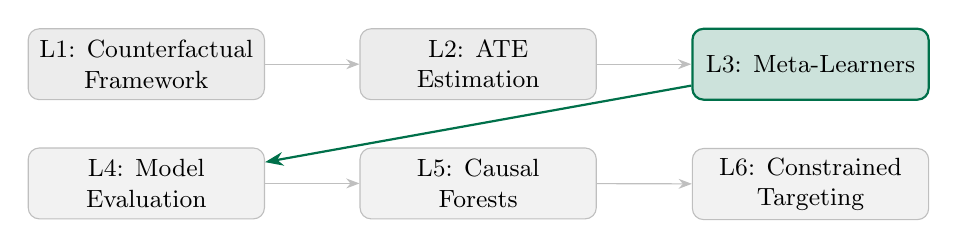
\begin{tikzpicture}[
    node distance=0.6cm and 1.2cm,
    box/.style={draw, rounded corners, minimum width=3cm, minimum height=0.9cm, font=\small, align=center},
    done/.style={box, fill=gray!15, draw=gray!50},
    active/.style={box, fill=sbgreen!20, draw=sbgreen, thick},
    inactive/.style={box, fill=gray!10, draw=gray!50}
]
\node[done] (L1) {L1: Counterfactual\\Framework};
\node[done, right=of L1] (L2) {L2: ATE\\Estimation};
\node[active, right=of L2] (L3) {L3: Meta-Learners};
\node[inactive, below=of L1] (L4) {L4: Model\\Evaluation};
\node[inactive, below=of L2] (L5) {L5: Causal\\Forests};
\node[inactive, below=of L3] (L6) {L6: Constrained\\Targeting};

\draw[-{Stealth}, gray!50] (L1) -- (L2);
\draw[-{Stealth}, gray!50] (L2) -- (L3);
\draw[-{Stealth}, thick, sbgreen] (L3) -- (L4);
\draw[-{Stealth}, gray!50] (L4) -- (L5);
\draw[-{Stealth}, gray!50] (L5) -- (L6);
\end{tikzpicture}
\end{center}
\end{frame}

% ====================================================================
\begin{frame}{Today's Plan}

\textbf{CATE Estimation with Meta-Learners}
\begin{enumerate}
    \item The CATE and the modeling problem
    \item The linear model with interactions (recap)
    \item S-Learner: one model with $D$ as feature
    \item T-Learner: two separate models
    \item The parameter-sharing spectrum
\end{enumerate}

\bigskip

\textbf{Next time (Lecture 4):} Model Evaluation -- Qini curves, AUUC, RATE, calibration, policy value, honest evaluation.

\end{frame}

% %%%%%%%%%%%%%%%%%%%%%%%%%%%%%%%%%%%%%%%%%%%%%%%%%%%%%%%%%%%%%%%%%%%%
% SESSION 1: CATE ESTIMATION WITH META-LEARNERS
% %%%%%%%%%%%%%%%%%%%%%%%%%%%%%%%%%%%%%%%%%%%%%%%%%%%%%%%%%%%%%%%%%%%%
 
% ====================================================================
\section{The CATE}
% ====================================================================
 
\begin{frame}{Recap: The CATE}
 
From Lecture 2:
 
\begin{block}{Conditional Average Treatment Effect (CATE)}
\[
\tau(x) = \E[Y(1) - Y(0) \mid X = x]
\]
\end{block}
 
The CATE is a \emph{function} of $x$, not a single number.
 
\bigskip
 
The ATE is its average: $\tau = \E[\tau(X)]$.
 
\bigskip
 
\textbf{Key difference from ATE:} the ATE asks ``does the treatment work on average?'' The CATE asks ``for whom does it work, and by how much?''
\end{frame}
 
% ====================================================================
\begin{frame}{CATE in Practice}
 
The CATE shows up whenever the treatment works differently for different people.
 
\bigskip
 
\textbf{Starbucks coupons:} the coupon lifts purchase probability by 20 pp for analysts but only 5 pp for executives. $X$ = customer type.
 
\bigskip
 
\textbf{Ride-hailing pricing:} a \textyen\,5 discount increases trip completion by 12\% for leisure riders but only 3\% for commuters. $X$ = trip purpose.
 
\bigskip
 
\textbf{Online advertising:} a display ad lifts conversion by 8\% for users unfamiliar with the brand but 0.5\% for existing customers. $X$ = prior brand exposure.
 
\bigskip
\pause
 
\textbf{Discussion:} Can you think of a setting where the CATE would be \emph{negative} for some subgroup? What would that mean for the targeting decision?
\end{frame}
 
% ====================================================================
\begin{frame}{Identification of the CATE}
 
How do we go from potential outcomes ($\tau(x) = \E[Y(1) - Y(0) \mid X = x]$) to something we can estimate from data?
 
\bigskip
 
\begin{block}{Theorem (Identification of the CATE)}
Under (1) SUTVA, (2) independence: $D \indep (Y(1), Y(0)) \mid X$, and (3) overlap: $0 < \Prob(D = 1 \mid X = x) < 1$ for all $x$:
\[
\tau(x) = \E[Y \mid D = 1, X = x] \;-\; \E[Y \mid D = 0, X = x]
\]
\end{block}
 
\bigskip
 
\textbf{Proof.} By consistency: $\E[Y \mid D\!=\!1, X\!=\!x] = \E[Y(1) \mid D\!=\!1, X\!=\!x]$.
 
By independence: $\E[Y(1) \mid D\!=\!1, X\!=\!x] = \E[Y(1) \mid X\!=\!x]$.
 
Analogously for $D = 0$. Subtract. $\square$
 
\bigskip
 
This is the CATE analog of the ATE identification from Lecture 2.
\end{frame}
 
% ====================================================================
\begin{frame}{The Overlap Assumption}
 
Independence says treatment is ``as good as random'' given $X$.
 
\bigskip
 
\textbf{Overlap} says: for every type of customer $x$, there must be \emph{some} treated and \emph{some} control observations.
 
\[
0 < \Prob(D = 1 \mid X = x) < 1 \quad \text{for all } x
\]
 
\bigskip
 
Without overlap, the CATE is still well-defined, but may not be properly identified/estimated from the data.
 
\bigskip
 
\textbf{Example:} Starbucks runs an A/B test only among loyalty members. For non-members, $\Prob(D = 1 \mid X = \text{non-member}) = 0$. We never observe a treated non-member, so any estimate of $\mu_1(\text{non-member})$ is extrapolation, not a data-driven comparison.
\end{frame}
 
% ====================================================================
\begin{frame}{Discussion: Do the Assumptions Hold?}
 
For each scenario, decide: does \textbf{independence} hold? Does \textbf{overlap} hold? What can we learn?
 
\bigskip
 
\begin{enumerate}
    \item \textbf{A/B test within loyal customers only}, random 50/50 within that group. Non-loyals are excluded.
 
    \medskip
 
    \item \textbf{Stratified A/B test:} gold-tier customers get the coupon with probability 70\%; silver-tier with probability 30\%. Assignment is random within each tier.
 
    \medskip
 
    \item \textbf{Coupons sent to customers who filed a complaint} in the past month; non-complainers get nothing.
 
    \medskip
 
    \item \textbf{Ride-hailing surge pricing} activated in high-demand zones; low-demand zones keep base price.
\end{enumerate}
 
\bigskip
\pause
 
\textcolor{gray}{\footnotesize Hint: for each, ask two questions. (a) Among the people you observe in treatment and control, is assignment independent of potential outcomes? (b) Are there subgroups where everyone (or no one) is treated?}
\end{frame}
 
% ====================================================================
\begin{frame}{Discussion: Answers}
 
\begin{center}
\small
\begin{tabular}{p{3.5cm}ccp{4.5cm}}
\toprule
\textbf{Scenario} & \textbf{Indep.} & \textbf{Overlap} & \textbf{What can we learn?} \\
\midrule
A/B within loyals & \textcolor{sbgreen}{Yes} & \textcolor{warnred}{Loyals only} & $\tau(x)$ for loyals; non-loyal CATEs are extrapolation \\[0.5em]
Stratified 70/30 & \textcolor{sbgreen}{Yes} & \textcolor{sbgreen}{Yes} & $\tau(x)$ for all $x$, but $e(x) \neq 0.5$ so naive $\bar{Y}_1 - \bar{Y}_0$ is biased for ATE \\[0.5em]
Coupons to complainers & \textcolor{warnred}{No} & \textcolor{warnred}{No} & Neither; complaint correlates with outcomes \\[0.5em]
Surge in high-demand & \textcolor{warnred}{No} & \textcolor{warnred}{Partial} & Neither; demand confounds price and outcomes \\
\bottomrule
\end{tabular}
\end{center}
 
\bigskip
 
Scenario 1 connects to the ATT $\neq$ ATE discussion from Lecture 2.

\end{frame}
 
% ====================================================================
\begin{frame}{From Identification to Estimation}
 
Identification gives us:
\[
\tau(x) = \underbrace{\E[Y \mid D = 1, X = x]}_{\mu_1(x)} \;-\; \underbrace{\E[Y \mid D = 0, X = x]}_{\mu_0(x)}
\]
 
\bigskip
 
\textbf{Two functions to estimate.} How hard is this?
 
\bigskip
 
With two customer types (exec, analyst): trivial. Compute within-group means.
 
\bigskip
 
With 10,000 customers and dozens of continuous features: we need a \textbf{model} for $\mu_1(x)$ and $\mu_0(x)$.
 
\bigskip
 
We start with the linear model, then generalize.
\end{frame}
 
 
% ====================================================================
\section{The Linear CATE Model}
% ====================================================================
 
\begin{frame}{Constant vs.\ Heterogeneous Effect}
 
\textbf{Constant effect model} (ANCOVA from Lecture 2):
\[
Y_i = \alpha + \tau D_i + \beta X_i + \varepsilon_i \quad \Longrightarrow \quad \tau(x) = \tau \text{ for all } x
\]
$X$ is treated as purely prognostic: affects the \emph{level} but not the \emph{effect}.
 
\bigskip
\pause
 
\textbf{Heterogeneous effect model} (add an interaction):
\[
Y_i = \alpha + \tau D_i + \beta X_i + \gamma (D_i \times X_i) + \varepsilon_i
\]
 
\[
\Longrightarrow \quad \tau(x) = \tau + \gamma \, x
\]
 
\bigskip
 
$\gamma \neq 0$ means $X$ changes the treatment effect. $\beta$ captures the baseline difference across types.
\end{frame}
 
% ====================================================================
\begin{frame}{Starbucks: The Interaction Model}
 
$X = 1$ (executive), $X = 0$ (analyst). Solving from the conditional expectations:
 
\[
\alpha = 0.10, \quad \tau = 0.20, \quad \beta = 0.65, \quad \gamma = -0.15
\]
 
\bigskip
 
CATEs:
\begin{itemize}
    \item $\tau(0) = \tau = 0.20$ (analysts)
    \item $\tau(1) = \tau + \gamma = 0.20 - 0.15 = 0.05$ (executives)
\end{itemize}
 
\bigskip
 
ATE $= \tau + \gamma \E[X] = 0.20 + (-0.15)(0.5) = 0.125$ $\checkmark$ 
 
\bigskip
 
The interaction coefficient $\gamma = -0.15$: being an executive reduces treatment effect by 15 pp. \\
The baseline difference between types ($\beta = 0.65$) is much larger.
\end{frame}
 
% ====================================================================
\begin{frame}{Limitations of the Linear Model}
 
\begin{enumerate}
    \item \textbf{Linearity:} CATE changes linearly with $X$. Exact for binary $X$; restrictive for continuous or high-dimensional $X$.
 
    \bigskip
 
    \item \textbf{Additivity:} covariates enter through additive, separable terms.
 
    \bigskip
 
    \item \textbf{Known specification:} the analyst must choose which interactions to include.
\end{enumerate}
 
\bigskip
 
When $X$ is high-dimensional or the CATE is nonlinear, we need more flexible methods.
 
\bigskip
 
\textbf{Idea:} replace OLS with any ML method. This gives us \textbf{meta-learners}.
\end{frame}
 
 
% ====================================================================
\section{Meta-Learners}
% ====================================================================
 
\begin{frame}{S-Learner: The Natural First Attempt}
 
The interaction model is already a ``single model with $D$ as a feature.'' Just replace OLS with a flexible learner:
 
\bigskip
 
\textbf{Algorithm:}
\begin{enumerate}
    \item Include $D$ as a \textbf{feature} alongside $X$
    \item Fit a single model: $\hat{f}(x, d) \approx \E[Y \mid X = x, D = d]$
    \item $\hat{\tau}(x) = \hat{f}(x, 1) - \hat{f}(x, 0)$
\end{enumerate}
 
\bigskip
 
``S'' for ``single.'' Uses all $n$ observations.
 
\bigskip
 
Any base learner works: random forest, XGBoost, neural network, \ldots
 
\bigskip
 
This is the most direct generalization of what we just did with OLS.
\end{frame}
 
% ====================================================================
\begin{frame}{S-Learner: The Regularization Bias}
 
\begin{alertblock}{Problem}
$D$ is one feature among many. A regularized model (LASSO, random forest, XGBoost) may \textbf{shrink its effect toward zero}.
\end{alertblock}
 
\bigskip
 
The treatment signal competes with covariate signal for the model's ``attention.''
 
\bigskip
 
In the extreme: LASSO sets all interaction coefficients to zero $\Rightarrow$ $\hat{\tau}(x) = \hat{\tau}$ for all $x$. The model predicts $Y$ well (captures prognostic variation) but misses the heterogeneity entirely.
 
\bigskip
\pause
 
\textbf{Can we do better?} What if we avoid the competition between $D$ and $X$ entirely?
\end{frame}
 
% ====================================================================
\begin{frame}{T-Learner: Separate the Arms}
 
\textbf{Idea:} don't make $D$ compete with $X$. Instead, fit two completely separate models:
 
\begin{center}
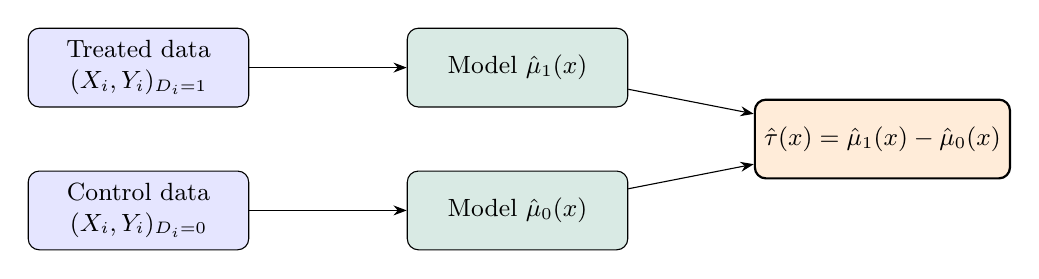
\begin{tikzpicture}[
    node distance=1.5cm and 2cm,
    box/.style={draw, rounded corners, minimum width=2.8cm, minimum height=1cm, font=\small, align=center},
    data/.style={box, fill=blue!10},
    model/.style={box, fill=sbgreen!15},
    result/.style={box, fill=orange!15, thick}
]
\node[data] (treat) {Treated data\\$(X_i, Y_i)_{D_i=1}$};
\node[data, below=0.8cm of treat] (ctrl) {Control data\\$(X_i, Y_i)_{D_i=0}$};
\node[model, right=of treat] (m1) {Model $\hat{\mu}_1(x)$};
\node[model, right=of ctrl] (m0) {Model $\hat{\mu}_0(x)$};
\node[result, right=3cm of $(m1)!0.5!(m0)$] (cate) {$\hat{\tau}(x) = \hat{\mu}_1(x) - \hat{\mu}_0(x)$};
 
\draw[-{Stealth}] (treat) -- (m1);
\draw[-{Stealth}] (ctrl) -- (m0);
\draw[-{Stealth}] (m1) -- (cate);
\draw[-{Stealth}] (m0) -- (cate);
\end{tikzpicture}
\end{center}
 
\bigskip
 
``T'' for ``two.'' Each model focuses on its own arm. No regularization can shrink the treatment effect, because $D$ never appears as a feature.
\end{frame}
 
% ====================================================================
\begin{frame}{T-Learner: The Variance Cost}
 
The T-learner solves the regularization bias. But it introduces a new problem:
 
\bigskip
 
\begin{alertblock}{Cost}
Each model sees only \textbf{half} the data. The two models are trained \textbf{independently}: no information sharing.
\end{alertblock}
 
\bigskip
 
If purchase history predicts outcomes similarly in both arms (prognostic variation), each model learns this pattern separately, wasting capacity.
 
\bigskip
 
Since the CATE is a \emph{difference}, errors in $\hat{\mu}_1$ and $\hat{\mu}_0$ accumulate rather than cancel.
 
\bigskip
\pause
 
The S-learner shared \emph{too much}. The T-learner shares \emph{nothing}. Is there a middle ground?
\end{frame}
 
% ====================================================================
\begin{frame}{Effect Modifiers vs.\ Prognostic Variables}
 
To understand the tradeoff, distinguish two kinds of covariates:
 
\bigskip
 
\textbf{Effect modifier:} a covariate $X_j$ such that $\tau(x)$ varies with $X_j$.
\begin{itemize}
    \item Customer type in Starbucks: $\tau(\text{analyst}) = 0.20 \neq 0.05 = \tau(\text{exec})$
    \item This is what we need for targeting
\end{itemize}
 
\bigskip
 
\textbf{Prognostic variable:} a covariate $X_j$ that predicts the outcome level $\E[Y \mid X]$ but does not change the treatment effect.
\begin{itemize}
    \item Commute distance: closer customers buy more, but the coupon effect is the same
    \item Helps with precision (ANCOVA from Lecture 2), not with targeting
\end{itemize}
 
\bigskip
 
The S-learner is good at prognostic variables but can miss effect modifiers. The T-learner detects effect modifiers but wastes capacity re-learning prognostic structure in each arm.
\end{frame}
 
% ====================================================================
\begin{frame}{The Parameter-Sharing Spectrum}
 
\begin{center}
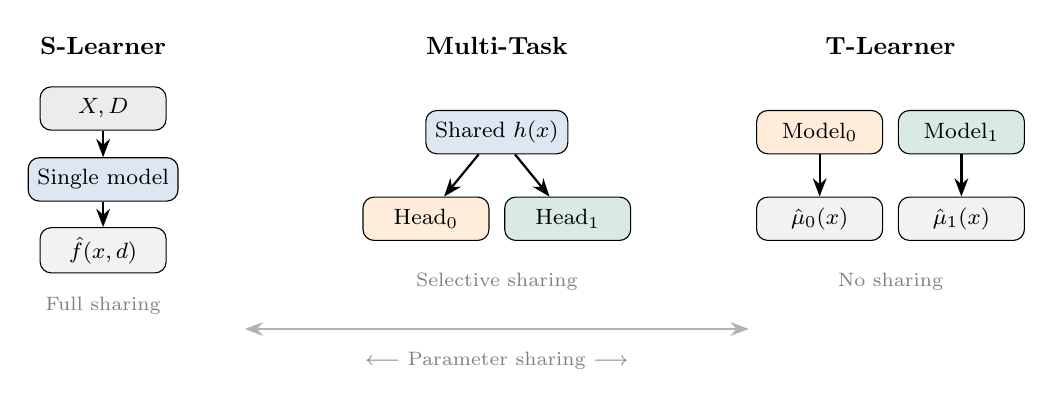
\begin{tikzpicture}[
    node distance=0.4cm and 0.8cm,
    layer/.style={draw, rounded corners, minimum width=1.6cm, minimum height=0.55cm, font=\footnotesize, align=center},
    input/.style={layer, fill=gray!15},
    shared/.style={layer, fill=noteblue!15},
    head0/.style={layer, fill=orange!15},
    head1/.style={layer, fill=sbgreen!15},
    output/.style={layer, fill=gray!10},
    arrow/.style={-{Stealth}, thick},
    title/.style={font=\small\bfseries, align=center}
]
 
% ── S-Learner ──
\node[title] at (0, 3.8) {S-Learner};
\node[input] (s-in) at (0, 3.0) {$X, D$};
\node[shared] (s-h1) at (0, 2.1) {Single model};
\node[output] (s-out) at (0, 1.2) {$\hat{f}(x,d)$};
\draw[arrow] (s-in) -- (s-h1);
\draw[arrow] (s-h1) -- (s-out);
\node[font=\scriptsize, text=gray] at (0, 0.5) {Full sharing};
 
% ── Multi-task ──
\node[title] at (5, 3.8) {Multi-Task};
\node[shared] (m-h1) at (5, 2.7) {Shared $h(x)$};
\node[head0] (m-head0) at (4.1, 1.6) {Head$_0$};
\node[head1] (m-head1) at (5.9, 1.6) {Head$_1$};
\draw[arrow] (m-h1) -- (m-head0);
\draw[arrow] (m-h1) -- (m-head1);
\node[font=\scriptsize, text=gray] at (5, 0.8) {Selective sharing};
 
% ── T-Learner ──
\node[title] at (10, 3.8) {T-Learner};
\node[head0] (t0-h1) at (9.1, 2.7) {Model$_0$};
\node[head1] (t1-h1) at (10.9, 2.7) {Model$_1$};
\node[output] (t0-out) at (9.1, 1.6) {$\hat{\mu}_0(x)$};
\node[output] (t1-out) at (10.9, 1.6) {$\hat{\mu}_1(x)$};
\draw[arrow] (t0-h1) -- (t0-out);
\draw[arrow] (t1-h1) -- (t1-out);
\node[font=\scriptsize, text=gray] at (10, 0.8) {No sharing};
 
% Spectrum arrow
\draw[{Stealth}-{Stealth}, thick, gray!60] (1.8, 0.2) -- (8.2, 0.2);
\node[font=\scriptsize, text=gray] at (5, -0.2) {$\longleftarrow$ Parameter sharing $\longrightarrow$};
\end{tikzpicture}
\end{center}
 
\bigskip
 
The \textbf{multi-task learner} (TARNet, DragonNet) is the middle ground: a shared representation $h(x)$ for the prognostic component, with separate output heads for $\mu_0$ and $\mu_1$.
\end{frame}
 
% ====================================================================
\begin{frame}{Bias-Variance Tradeoff across the Spectrum}
 
\begin{center}
\begin{tabular}{p{2.5cm}p{4.5cm}p{4.5cm}}
\toprule
& \textbf{Bias risk} & \textbf{Variance risk} \\
\midrule
\textbf{S-Learner} & High (regularization can mask effect modifiers) & Low (single model, all $n$) \\[0.8em]
\textbf{Multi-Task} & Moderate (heads have limited capacity) & Moderate (shared body uses all $n$) \\[0.8em]
\textbf{T-Learner} & Low (each arm unrestricted) & High ($n/2$ per model; prognostic structure learned twice) \\
\bottomrule
\end{tabular}
\end{center}
\end{frame}
 
% ====================================================================
\begin{frame}{Why the Spectrum Matters in Business Settings}
 
\textbf{Key insight:} most outcome variation in business settings is \emph{prognostic}.
 
\bigskip
 
Customer characteristics predict purchase levels strongly, but the treatment effect is a small perturbation on top.
 
\bigskip
 
\begin{itemize}
    \item \textbf{S-learner} shares everything, including the treatment-specific component. When $D$ contributes only a few percent of outcome variance, the model may decide $D$ is not worth attending to.
 
    \medskip
 
    \item \textbf{T-learner} estimates the large prognostic component independently in each arm, consuming most capacity on something that could be shared.
 
    \medskip
 
    \item \textbf{Multi-task} shares parameters for prognostic variation (where data is abundant) while keeping separate parameters for treatment effects (where flexibility matters).
\end{itemize}
\end{frame}
 
% ====================================================================
\begin{frame}{Summary: All Are Outcome Modeling}
 
\begin{center}
\begin{tabular}{p{2.5cm}p{4cm}p{4.5cm}}
\toprule
\textbf{Method} & \textbf{Strength} & \textbf{Weakness} \\
\midrule
\textbf{Linear model} & Simple, interpretable & Linearity; must specify interactions \\[0.6em]
\textbf{S-Learner} & All data; good at prognostics & Regularization shrinks effects \\[0.6em]
\textbf{T-Learner} & Flexible; detects effect modifiers & High variance; no sharing \\[0.6em]
\textbf{Multi-task} & Shares prognostic structure & More complex; needs large $n$ \\
\bottomrule
\end{tabular}
\end{center}
 
All four are \textbf{outcome modeling}: minimize prediction error for $Y$; the treatment effect falls out as a byproduct. None has a loss function that targets $\tau(x)$.  
 
\bigskip
 
An alternative: directly target $\tau(x)$. This is what causal forests do (Lecture 5).
\end{frame}


% ====================================================================
\begin{frame}{The Targeting Depth Curve}
 
Rank all customers by $\hat{\tau}(x_i)$ descending. As we expand the target set, the ATT falls:
 
\bigskip
 
\begin{center}
\begin{tabular}{lccc}
\toprule
\textbf{Depth} $k$ & \textbf{Who is targeted} & $\tau_{S_k}$ & \textbf{Interpretation} \\
\midrule
1,000 & Top 1,000 analysts & 0.20 & Highest-effect only \\
5,000 & All analysts & 0.20 & All high-effect customers \\
7,500 & Analysts $+$ 2,500 exec & 0.15 & Diluted by executives \\
10,000 & Everyone & 0.125 & $=$ ATE \\
\bottomrule
\end{tabular}
\end{center}
 
\bigskip
 
If the ranking is corrupted (noisy, biased), we treat the wrong people and $\tau_{S_k}$ is lower at every depth.
\end{frame}
 
% ====================================================================
\begin{frame}{Ranking Quality Is What Matters}
 
Sometimes, the business value of CATE estimation depends on how well $\hat{\tau}(x)$ \emph{ranks} customers, not on the accuracy of individual point estimates.
 
\bigskip
 
A model with correct rankings but wrong magnitudes produces a better targeting rule than a model with accurate magnitudes but poor rankings.
 
\bigskip
 
$\Rightarrow$ We need an \textbf{evaluation framework} for CATE rankings.
 
\end{frame}
 
% ====================================================================
\begin{frame}{Key Takeaways}
 
\begin{enumerate}
    \item The \textbf{CATE} $\tau(x) = \E[Y(1) - Y(0) \mid X = x]$ is identified under independence and overlap. Without overlap, estimates are extrapolation.
 
    \medskip
 
    \item The \textbf{S-Learner} is the natural first attempt: one model with $D$ as feature. Flexible, but regularization can shrink the treatment effect toward zero.
 
    \medskip
 
    \item The \textbf{T-Learner} fixes this by separating the arms. But it pays a variance cost: each model sees half the data and learns prognostic structure independently.
 
    \medskip
 
    \item These sit on a \textbf{parameter-sharing spectrum}. The multi-task learner shares the prognostic component while keeping treatment effects separate.
 
    \medskip
 
    \item All are \textbf{outcome modeling}: estimate $\mu_1, \mu_0$, subtract.
 
\end{enumerate}
\end{frame}

\end{document}
